\section{数据库概念设计}\label{sec:ConceptualDesign}

在本节(\cref{sec:ConceptualDesign})中,我们将介绍数据库实体及相关属性、数据库总体E-R图和数据库模块E-R图。

\subsection{数据库实体及相关属性}

在数据库设计中,模块划分是根据业务功能和逻辑结构进行的。具体划分为用户模块、宠物社区模块、宠物新闻模块、以及宠物百科与领养模块。每个模块负责特定的功能,如用户模块处理用户信息;宠物社区模块涉及社交互动,如帖子、评论和用户互动;宠物新闻模块管理新闻发布和用户反馈;宠物百科与领养模块则涉及宠物的详细信息管理和领养过程。

\subsubsection{用户模块}

用户模块相关的数据库实体及相关属性:

\begin{itemize}
    \item \textbf{用户表}(\underline{用户ID},用户名,密码,手机号码,注册日期,上次登录时间,用户角色,用户状态,头像链接,个人简介,性别,出生日期,经验点数,关注数,被关注数,收藏数,被收藏数,点赞数,被点赞数,留言数)
    \item \textbf{用户设置表}(\underline{用户ID},是否公开手机号码,是否公开注册日期,是否公开个人简介,是否公开性别,是否公开出生日期,是否公开等级,是否公开关注数,是否公开被关注数,是否公开收藏数,是否公开被收藏数,是否公开点赞数,是否公开被点赞数,是否公开留言数,是否允许他人关注,是否接受管理员通知,是否接受用户通知)
    \item \textbf{用户打卡表}(\underline{打卡记录ID},用户ID,打卡时间)
    \item \textbf{用户关注表}(\underline{被关注者ID},\underline{关注者ID},关注时间)
    \item \textbf{用户留言表}(\underline{留言ID},用户ID,留言者ID,留言内容,留言时间)
    \item \textbf{用户反馈表}(\underline{反馈意见ID},反馈类型,反馈内容,反馈时间,电子邮箱,手机号码)
\end{itemize}

\subsubsection{宠物社区模块}

宠物社区模块相关的数据库实体及相关属性:

\begin{itemize}
    \item \textbf{帖子分类表}(\underline{帖子分类ID},帖子分类)
    \item \textbf{帖子表}(\underline{帖子ID},发帖用户ID,帖子分类ID,标题,内容,创建时间,更新时间,是否置顶,点赞数,点踩数,收藏数,评论数,图片链接)
    \item \textbf{帖子评论表}(\underline{帖子评论ID},帖子ID,用户ID,父评论ID,评论内容,评论时间,点赞数,点踩数)
    \item \textbf{帖子点赞表}(\underline{帖子ID},\underline{用户ID},点赞时间)
    \item \textbf{帖子点踩表}(\underline{帖子ID},\underline{用户ID},点踩时间)
    \item \textbf{帖子评论点赞表}(\underline{帖子评论ID},\underline{用户ID},点赞时间)
    \item \textbf{帖子评论点踩表}(\underline{帖子评论ID},\underline{用户ID},点踩时间)
    \item \textbf{帖子收藏表}(\underline{帖子ID},\underline{用户ID},收藏时间)
    \item \textbf{帖子举报表}(\underline{帖子举报ID},举报者ID,被举报者ID,被举报帖子ID,举报原因,举报时间,处理状态)
    \item \textbf{帖子评论举报表}(\underline{帖子评论举报ID},举报者ID,被举报者ID,被举报评论所属帖子ID,被举报评论ID,举报原因,举报时间,处理状态)
\end{itemize}

\subsubsection{宠物新闻模块}

宠物新闻模块相关的数据库实体及相关属性:

\begin{itemize}
    \item \textbf{新闻标签表}(\underline{新闻标签ID},新闻标签)
    \item \textbf{新闻表}(\underline{新闻ID},管理员ID,新闻标签ID,标题,新闻摘要,内容,创建时间,更新时间,封面图片链接,是否置顶,点赞数,点踩数,收藏数,评论数)
    \item \textbf{新闻评论表}(\underline{新闻评论ID},新闻ID,用户ID,父评论ID,评论内容,评论时间,点赞数,点踩数)
    \item \textbf{新闻点赞表}(\underline{新闻ID},\underline{用户ID},点赞时间)
    \item \textbf{新闻点踩表}(\underline{新闻ID},\underline{用户ID},点踩时间)
    \item \textbf{新闻评论点赞表}(\underline{新闻评论ID},\underline{用户ID},点赞时间)
    \item \textbf{新闻评论点踩表}(\underline{新闻评论ID},\underline{用户ID},点踩时间)
    \item \textbf{新闻收藏表}(\underline{新闻ID},\underline{用户ID},收藏时间)
    \item \textbf{新闻评论举报表}(\underline{新闻评论举报ID},举报者ID,被举报者ID,被举报评论所属新闻ID,被举报评论ID,举报原因,举报时间,处理状态)
\end{itemize}

\subsubsection{宠物百科与领养模块}

宠物百科模块相关的数据库实体及相关属性:

\begin{itemize}
    \item \textbf{宠物分类表}(\underline{宠物分类ID},宠物分类名称(十种语言),描述(十种语言),图片链接)
    \item \textbf{宠物子类表}(\underline{宠物子类ID},宠物分类ID,宠物子类名称(十种语言),描述(十种语言),图片链接,起源地(十种语言),体型(十种语言),毛色(十种语言),寿命(十种语言),性情(十种语言),饮食习惯(十种语言),经纬度参数)
    \item \textbf{宠物护理指导表}(\underline{宠物护理指导ID},宠物子类ID,标题(十种语言),内容(十种语言))
    \item \textbf{宠物领养表}(\underline{宠物领养ID},用户ID,宠物分类ID,宠物子类ID,宠物名称,图片链接,宠物年龄,地址,转让原因,健康情况,最近一次健康检查日期,疫苗接种情况,特殊护理需求,特殊饮食需求,性格行为特征,是否已绝育,备注,领养状态,性别,附件链接)
\end{itemize}

\subsubsection{开发团队模块}

开发团队模块相关的数据库实体及相关属性:

\begin{itemize}
    \item \textbf{开发团队表}(\underline{学号},姓名,学校,电子邮箱,Github名称,Github主页)
\end{itemize}

\subsection{数据库总体E-R图}

数据库总体E-R图见\cref{fig:GeneralERDiagram}。

\begin{figure}[htbp]
    \centering
    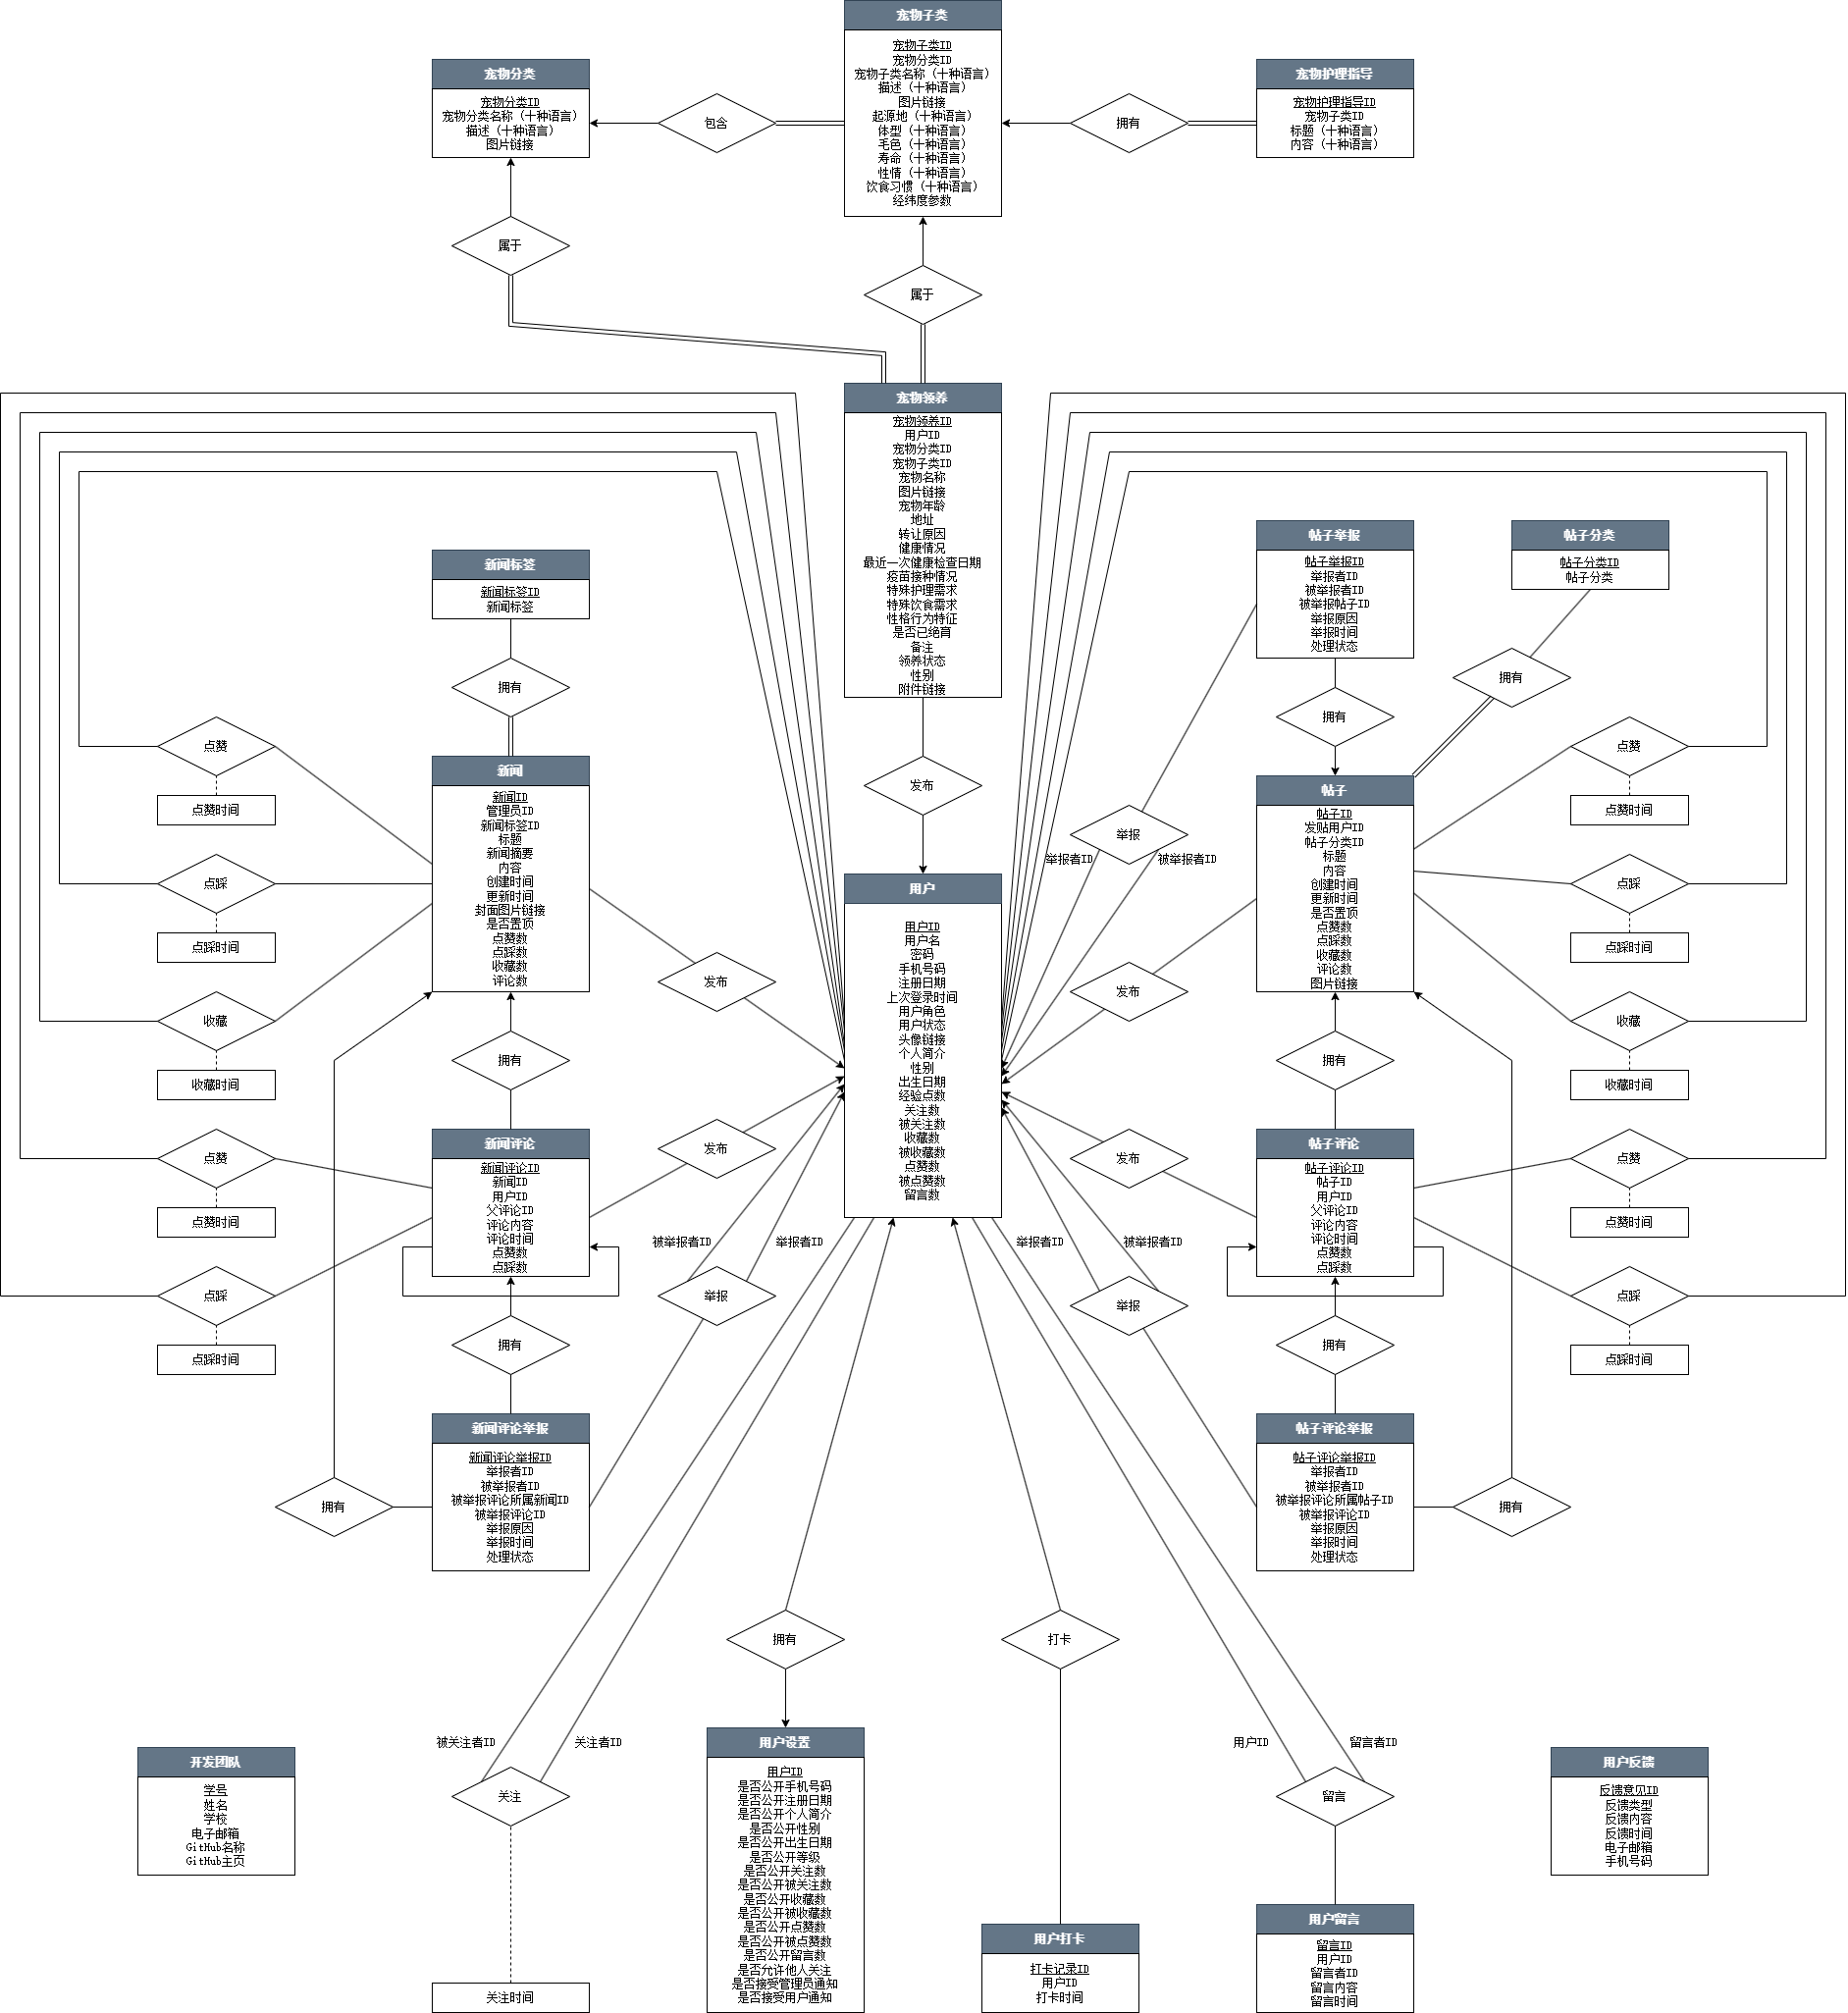
\includegraphics[width=\textwidth]{figures/GeneralERDiagram.png}
    \caption{数据库总体E-R图}
    \label{fig:GeneralERDiagram}
\end{figure}

数据库的总体E-R图是设计的宏观视图,展示了所有主要实体及其关系。这个图包括了用户、帖子、新闻、宠物分类、宠物子类等实体,以及它们之间的关系如一对多、多对多关系。例如,用户与帖子之间的多对一关系(一个用户可以发布多个帖子),帖子与评论之间的一对多关系(一个帖子可以有多个评论)。总体E-R图还明确展示了如用户设置、用户关注、用户留言、新闻评论等更细致的功能关系。通过这样的设计,可以清楚地理解数据库的结构和各部分之间的交互,为数据库的实际建设和未来的数据操作提供明确的指导。

\subsection{数据库模块E-R图}

\subsubsection{用户模块E-R图}

用户模块的E-R图设计专注于维护用户的基本信息和用户间的互动。核心实体包括用户表,用户设置表,用户打卡表,用户关注表,用户留言表。用户表存储所有注册用户的详细信息,如用户名、密码、联系方式等,同时提供唯一标识符来关联其他表中的用户活动和设置。用户设置表与用户表具有一对一关系,记录用户的个性化设置如隐私偏好和通知接收偏好。用户打卡表、用户关注表和用户留言表则描述用户的社交互动,展示了用户间如何互动和通信。

用户模块E-R图见\cref{fig:UserERDiagram}。

\begin{figure}[htbp]
    \centering
    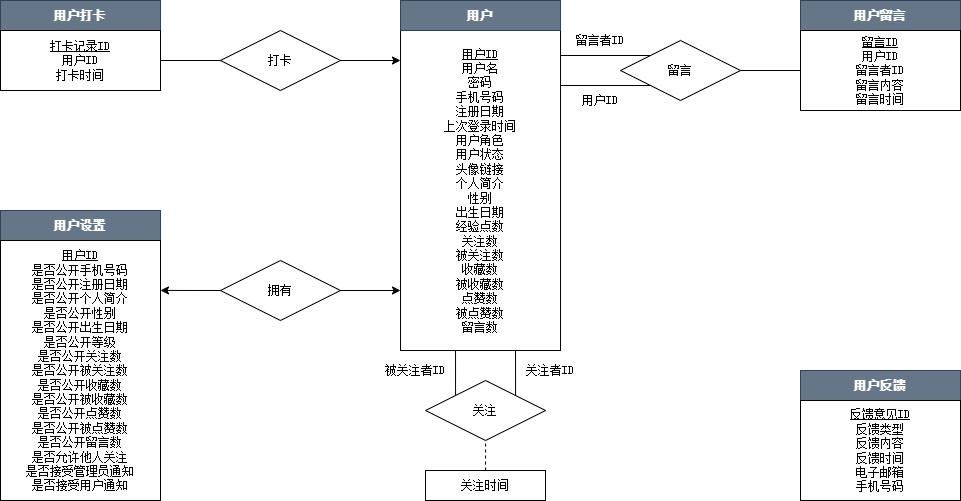
\includegraphics[width=\textwidth]{figures/UserERDiagram.png}
    \caption{用户模块E-R图}
    \label{fig:UserERDiagram}
\end{figure}

\subsubsection{宠物社区模块E-R图}

宠物社区模块的E-R图设计专注于处理与社区相关的用户互动,例如帖子的发布、评论、点赞、点踩、收藏以及举报等功能。此模块包括帖子表、帖子评论表、帖子点赞和点踩表、帖子收藏表以及帖子和评论的举报表。每个帖子可以有多个评论、多个点赞、多个点踩、多个收藏,并且可以被多次举报。用户可以发表帖子、对帖子进行评论和对评论进行回复。此外,E-R图展示了用户与帖子及其交互之间的关系,如用户和帖子之间的发布关系、用户与点赞或点踩之间的关系。设计的重点在于明确和组织用户互动的数据结构,确保用户行为的追踪和管理,以便为社区成员提供丰富且互动的用户体验。

宠物社区模块E-R图见\cref{fig:PetCommunityERDiagram}。

\begin{figure}[htbp]
    \centering
    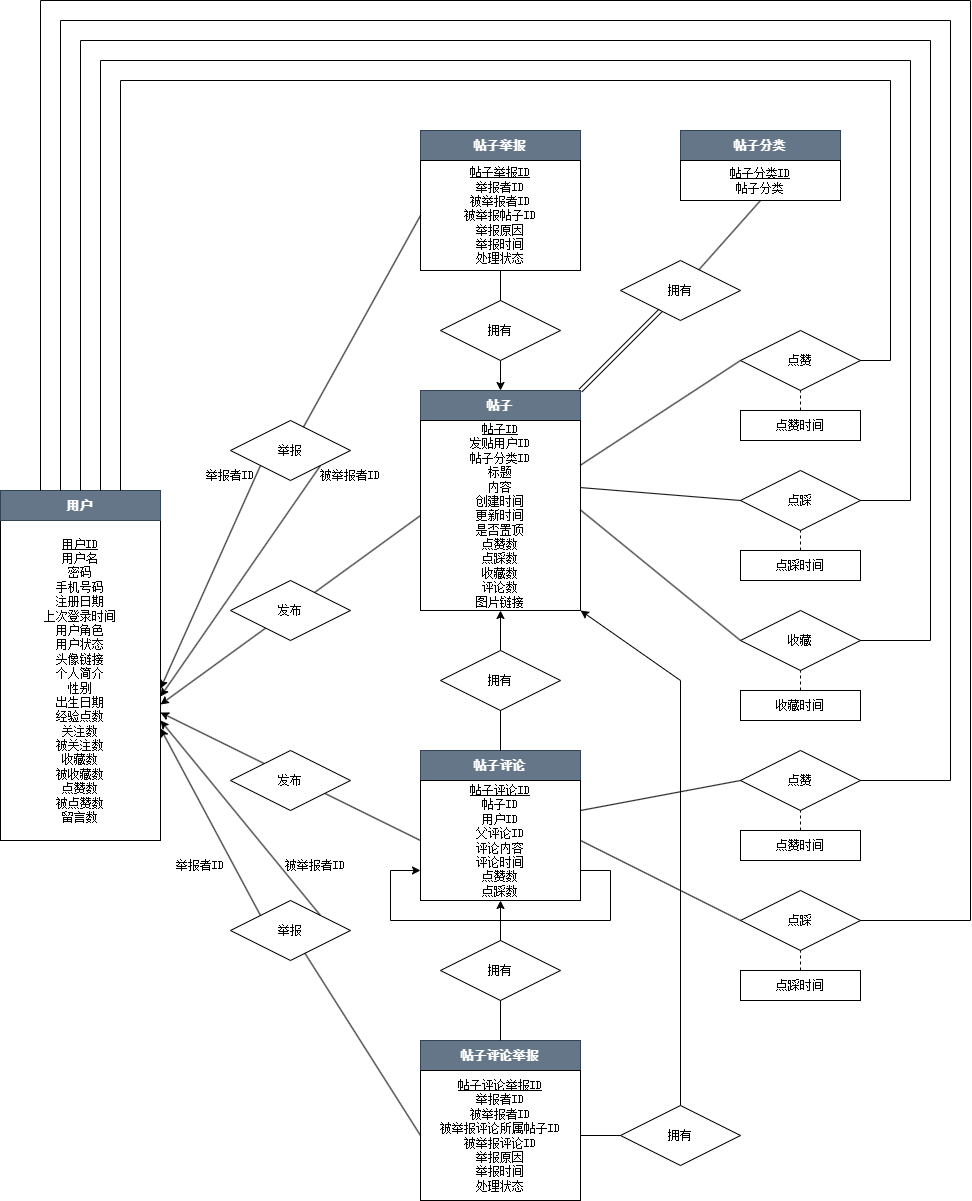
\includegraphics[width=\textwidth]{figures/PetCommunityERDiagram.png}
    \caption{宠物社区模块E-R图}
    \label{fig:PetCommunityERDiagram}
\end{figure}

\subsubsection{宠物新闻模块E-R图}

宠物新闻模块的E-R图设计关注于管理和展示新闻内容及其用户互动,包括新闻的发布、评论、点赞、点踩、收藏以及评论的举报。核心实体包括新闻表、新闻评论表、新闻点赞表、新闻点踩表、新闻收藏表和新闻评论举报表。新闻表与新闻标签表连接,表明每条新闻都归属于特定的新闻标签。新闻与用户的互动如评论、点赞、点踩和收藏通过一对多关系实现,每个新闻可以有多个评论和多次点赞或点踩,而每条评论也可以被多个用户点赞或点踩。此外,新闻和评论的举报功能允许用户报告不适当的内容,增强社区的内容管理效率。这个设计旨在确保新闻内容的有效管理和用户交互的流畅性,同时提供一个结构清晰、易于维护的数据库模型。

宠物新闻模块E-R图见\cref{fig:PetNewsERDiagram}。

\begin{figure}[htbp]
    \centering
    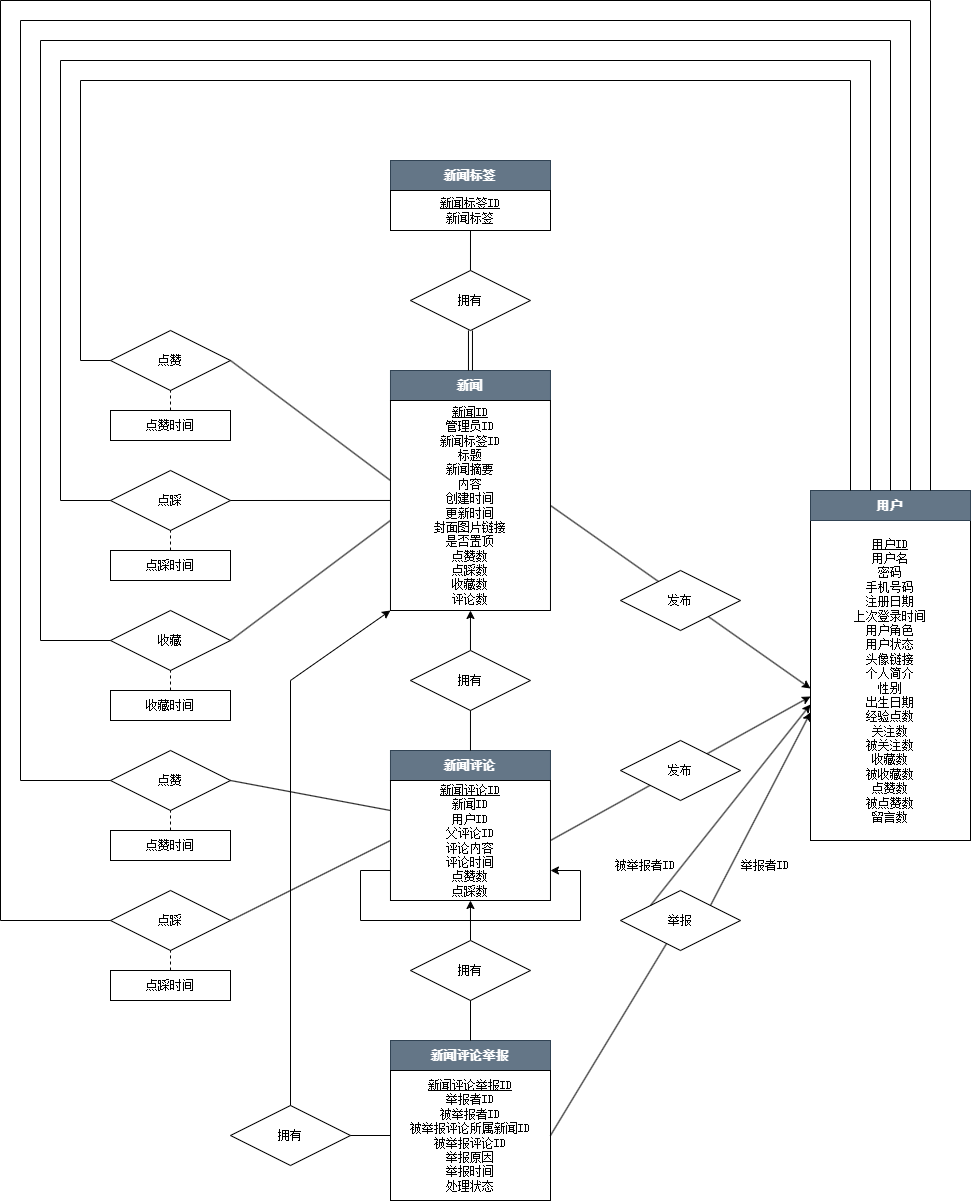
\includegraphics[width=\textwidth]{figures/PetNewsERDiagram.png}
    \caption{宠物新闻模块E-R图}
    \label{fig:PetNewsERDiagram}
\end{figure}

\subsubsection{宠物百科与领养模块E-R图}

宠物百科与领养模块的E-R图设计旨在详细管理宠物相关信息以及领养过程中的所有数据交互。这个模块包括宠物分类表、宠物子类表、宠物护理指导表以及宠物领养表等实体。宠物分类与子类之间的关系是一对多,表示一个宠物分类包含多个子类,例如犬类包括不同的狗种。每个宠物子类还关联到具体的护理指导,以提供针对性的护理信息。宠物领养表核心连接用户与宠物,每个领养记录关联一个用户和一个具体的宠物子类,确保领养过程中的信息一致性和完整性。此外,每个领养记录详细记录了宠物的健康状况、位置、年龄等关键信息。这个设计不仅有助于用户轻松获取宠物的详细信息和护理指南,还促进了透明和规范的宠物领养流程。

宠物百科与领养模块E-R图见\cref{fig:PetEncyclopediaAndAdoptionERDiagram}。

\begin{figure}[htbp]
    \centering
    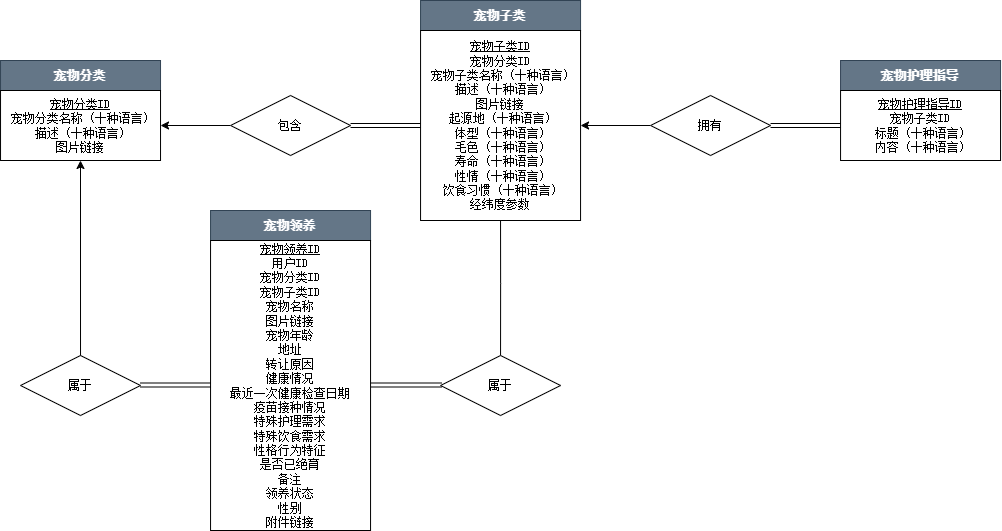
\includegraphics[width=\textwidth]{figures/PetEncyclopediaAndAdoptionERDiagram.png}
    \caption{宠物百科与领养模块E-R图}
    \label{fig:PetEncyclopediaAndAdoptionERDiagram}
\end{figure}

\subsubsection{开发团队模块E-R图}

开发模块的E-R图设计相对简单,因为它主要涉及一个单独的表——开发团队表(DEVELOPMENT\_TEAM),该表用于存储开发团队成员的详细信息。这个表是独立的,不与数据库中的其他实体或表直接关联。其设计目的主要是为了在应用或网站的“关于宠悦”界面上展示开发团队的信息,如成员姓名、学号、学校、电子邮箱、GitHub名称和GitHub主页等。

开发团队模块E-R图见\cref{fig:DevelopmentTeamERDiagram}。

\begin{figure}[htbp]
    \centering
    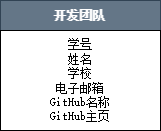
\includegraphics[width=0.2\textwidth]{figures/DevelopmentTeamERDiagram.png}
    \caption{开发团队模块E-R图}
    \label{fig:DevelopmentTeamERDiagram}
\end{figure}

在E-R图中,开发团队表被展示为一个单独的实体,具有自己的属性:

\begin{itemize}
    \item \textbf{主键}:学号(id)
    \item \textbf{其他属性}:姓名(name)、学校(school)、电子邮箱(email)、GitHub名称(github\_name)、GitHub主页(github\_profile)
\end{itemize}

由于该表没有与其他表的关系,E-R图中不会显示任何连接线或外键关联。这种设计强调了表的独立性和特定用途,即仅用于信息展示而不参与系统的其他功能或逻辑处理。这样的设计也有利于简化数据库维护和数据管理,因为它不涉及复杂的关系处理,只需关注信息的准确性和更新。